% !TeX spellcheck = en_US
\chapter{Introduction}\label{intro}%


	
	%	Our work presents a model-based approach to automate the creation of reliable E/E network architectures in such a way that it can automatically create single and high-redundant routes for non-safety and safety-critical applications, respectively, based on predetermined optimization objectives (i.e., cost and allocated links optimization).
	
	
	
    \section{Vehicle E/E Architecture and its Development}\label{eeArch}
    %Almost all aspects of E/E system development including technical approaches, specified requirements, decision-making about design structure, and developments methods are affected by vehicle E/E architecture. Vehicle architecture can be seen from various perspectives. The physical vision illustrates the positioning and the connection of the used elements in the car such as ECUs, sensors, actuators, gateways, power supply, and switches. Moreover, it includes communication networks, wiring harness placement, and power distribution setup. In addition, the automotive software plays a pivotal role in the vehicle E/E architecture since the autonomous level of cars has been improving in the last decade. 
    The automotive industry is profoundly transforming, driven by technological advancements and a growing emphasis on safety, connectivity, and automation. Central to these changes is the concept of electrical and/or electronic (E/E) architecture, which refers to the organizational structure and integration of electrical and electronic systems within a vehicle.
    The development of E/E systems, including the technical approaches, requirements, design structure decisions, and methods, are heavily influenced by the vehicle's E/E architecture~\cite{9565115,askaripoor2023designer}. 
    
    The E/E architecture can be viewed from multiple perspectives. One is the physical aspect that shows the positioning and connections of elements in the car, such as electronic control units (ECUs), sensors, actuators, gateways, power supply, and switches. It also includes the placement of communication networks, wiring harnesses, and power distribution setups. Furthermore, the software used in the vehicle plays a crucial role in the E/E architecture, especially as the level of autonomy in cars has been advancing in recent years.
    %Another perspective of E/E architecture is logical vision so that the focus is the interaction and interconnection among various components and elements integrated into the car. Based on this point of view, the E/E architecture can be interpreted to be about data exchange, signal flows, and communication and interface protocols. 
    Another perspective is that the E/E architecture can be seen as a logical representation, emphasizing the connection and interaction between the components and elements incorporated into the vehicle. In this context, the E/E architecture can be understood as pertaining to the transfer of data, the movement of signals, and the protocols for communication and interfaces~\cite{askaripoor2022architecture}.
    
    %The level of driving automation has been improving in recent years, and a lot of companies have spent a huge amount of effort as well as cost to move towards an autonomous vehicle. This has enabled vehicles to provide not only non-critical functionalities and features, e.g., gaming using vehicle infotainment system but also giving ADAS functionalities to drivers to have safe and more comfortable driving experiences. Accordingly, the automotive E/E architecture has advanced significantly, from various sensors and actuators to more powerful computing units to process a huge amount of data coming from the sensors for critical and non-critical functionalities~\cite{bandur2021making}.
    Recent advancements in driving automation have led to a significant increase in the number of companies investing in the development of autonomous vehicles. This effort has not only resulted in the inclusion of non-essential features, such as gaming using a vehicle's infotainment system, but also the implementation of advanced driver assistance systems (ADAS) to enhance safety and comfort for drivers. As a result, the E/E architecture of automobiles has undergone significant improvements, including the integration of various sensors, actuators, and powerful computing units to process the large amounts of data collected from the sensors for both critical and non-critical functions~\cite{askaripoor2022architecture}.
    
    
    %With increasing the number of functionalities and features, the vehicle E/E architecture has been altering during the last years. The car ECU starts as function-specific, where each ECU handles each function. Domain-specific ECU represents the next level of controllers where a computer controls a set of functions related to a specific area or domain. Functional domains that require a domain ECU are typically compute-intensive and connect to a large number of input/output (I/O) devices. Each domain ECU connects to multiple function-specific control units. A zonal ECU provides and distributes data and power; in other words, the vehicle battery power is diffused over the car architecture, e.g., for running various sensors and actuators, using zonal controllers. Similarly, the data is spread over vehicle's network and transferred from sensors to other actuators/sensors and controllers using zonal ECUs. In addition, this type of ECU supports any feature available in the specific vehicle zone and it acts as a gateway, switch, and as a smart junction box. Moreover, it supports any kind of interface for sensors, actuators, and displays. 
    
    Over the past few years, as the number of functionalities and features in vehicles has grown, the E/E architecture of cars has undergone significant changes~\cite{9212001}. Initially, each ECU was responsible for managing a single function. As the number of functions increased, domain-specific ECUs emerged, responsible for controlling a set of functions related to a specific area or domain. These functional domains that require domain ECUs are usually compute-intensive and connect to many input/output (I/O) devices~\cite{9613692}. Each domain ECU is connected to multiple function-specific control units. A zonal ECU is responsible for distributing data and power throughout the vehicle, for example, by distributing the power from the vehicle battery to various sensors and actuators using zonal controllers.
    Similarly, data is spread over the vehicle's network and transferred from sensors to other actuators/sensors and controllers using zonal ECUs. In addition, this type of ECU supports any feature available in the specific vehicle zone and acts as a gateway, switch, and smart junction box. Furthermore, it supports any interface for sensors, actuators, and displays~\cite{askaripoor2023designer, askaripoor2022architecture}.
    
    
    
    %The central HPCU is a multi-core ECU which comprises a multi-system on chips (SoCs) (each includes several cores), graphics processing unit (GPU), random access memory (RAM), and deep learning accelerators to process high computational power-demand applications such as various object detection applications used for ADAS functionalities~\cite{9613692}. The central computing unit is a fully scalable and upgradeable platform that connects to Edge and Cloud back-end and uses cloud computing for processing intensive vehicle functionalities. Furthermore, it can function as the zonal gateway. In other words, this ECU functions as the master and the core functionality of the vehicle
    Considering the ADAS and self-driving applications, using domain-specific ECUs increases the number of ECUs with substantial growth in the wiring harness, communication bandwidth, cost, software variants, and software complexity. Therefore, multi-core ECUs can be considered a solution to reduce the number of ECUs, cost, wiring harness, software complication, and variations. In addition, the multi-core technology has promptly been extending in different areas of embedded systems to deliver an appropriate performance for artificial intelligence (AI)-based applications and systems by giving scalable computing power~\cite{broy2006challenges,askaripoor2022architecture}.
    A high-performance computing unit (HPCU) is a multi-core ECU that is composed of multiple system on chips (SoCs) that include several cores, a graphics processing unit (GPU), random access memory (RAM), and deep learning accelerators. These components work together to process high computational power-demand applications such as various object detection applications for ADAS functionalities~\cite{9613692}. The central computing unit is a fully scalable and upgradeable platform that connects to Edge and Cloud backend and uses cloud computing to process intensive vehicle functionalities. Additionally, it can act as the zonal gateway, meaning it serves as the master and core functionality of the vehicle~\cite{askaripoor2022architecture}. 
    
    \begin{figure}[t]
    \centering
    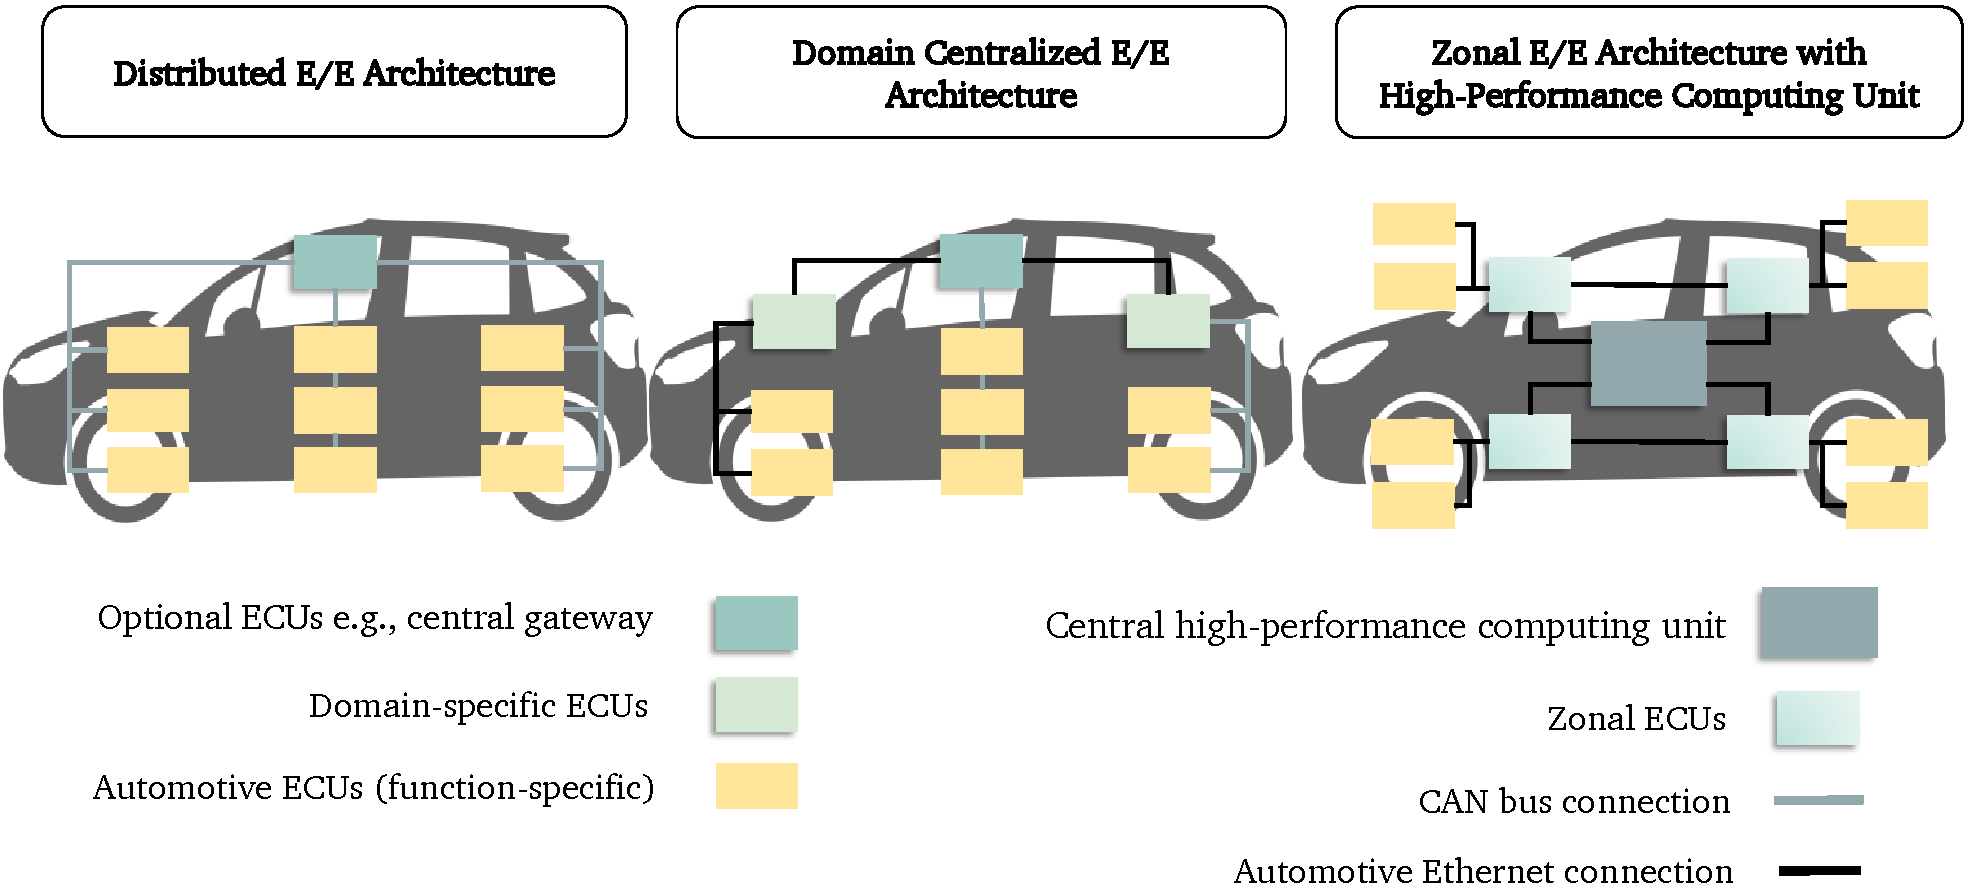
\includegraphics[width=1\textwidth]{figures/eearch1.pdf}
    \caption{The figure presents the evolution of vehicle E/E architecture. Distributed E/E architectures were used until 2019, while domain-centralized architectures are used nowadays as vehicle architectures. The zonal architecture shows the future car E/E architecture~\cite{askaripoor2022architecture}.}
    \label{fig011}
    \end{figure}
    
    %Figure.~\ref{fig1} shows the progress of E/E architectures. It starts from distributed E/E architecture, which consists of function-specific ECUs and a central gateway which are connected via controller area network (CAN) bus. Utilizing the central gateway provides stronger collaboration among ECUs, the ability to handle more complex functions, e.g., adaptive cruise control, and the potential of cross-functional connection. The next evolution represents domain centralized E/E architectures which utilize domain-specific ECUs \cite{apostu2019automotive}. As Figure.~\ref{fig1} shows function-specific control units bind to domain-specific ECUs using a CAN bus and Ethernet connection. Moreover, the central gateway ECU is used in this type of architecture~\cite{butzkamm_brand_2020}. This architecture is capable of handling more complex functions; furthermore, the architecture cost can be optimized using the consolidation of the functions. For instance, one domain-specific ECU is assigned for the parking assistance system which includes two function-specific controllers related to vision processing and actuator commands, e.g., for brake and steering wheel. 
    
    As shown in Figure~\ref{fig011}, the development of E/E architectures has progressed through various stages. The initial stage referred to as distributed E/E architecture, involves using function-specific ECUs and a central gateway connected via a controller area network (CAN) bus. This architecture allows for stronger collaboration among ECUs and the ability to handle more complex functions, such as adaptive cruise control, as well as the potential for cross-functional connections. The next evolution in E/E architecture is known as domain centralized architecture, which utilizes domain-specific ECUs~\cite{askaripoor2022architecture}. As shown in Figure~\ref{fig011}, function-specific control units are connected to domain-specific ECUs using both a CAN bus and an Ethernet connection. Moreover, this type of architecture also utilizes the central gateway ECU. This architecture is capable of handling even more complex functions and can also optimize cost through the consolidation of functions. For example, one domain-specific ECU can be assigned for the parking assistance system, which includes two function-specific controllers related to vision processing and actuator commands, such as for brake and steering wheel~\cite{askaripoor2022architecture}.
    
    
    
     %Domain centralized architecture, using domain controllers and central gateway, has grown over time and become extremely elaborate, including the car wiring harness. Furthermore, the autonomous driving feature significantly increases the complexity of the architecture because of the increase in the number of sensors and actuators, growth of data processing capabilities and required bandwidth and high demand for intelligent power distribution~\cite{zerfowski2019functional}. The future E/E architecture, which is a zonal architecture, can deal with the existed complexity in the last two architectures using the central HPCU~\cite{Zonal}. 
     %The zonal architecture blends future vehicle functions and technologies with savings in weight and cost. As Figure~\ref{fig1} presents, the zonal architecture comprises a HPCU, zonal ECUs, and function-specific ECUs. The central HPCU acts as the master to process all data coming from different vehicle zones and consequently operate the car. In addition, the HPCU functions as a central gateway to pass the data from one zone to another~\cite{jiang2019vehicle}. The ECUs and HPCU are interconnected via the Ethernet connection for transmitting the data over the vehicle's network because of its speed and high bandwidth for data transmission~\cite{apostu2019automotive}. More importantly, the zonal architecture supports the virtual domain in such a way that the embedded functions can be transferred into the cloud as well as providing software download/update via update over the air (OTA) service for HPCU~\cite{shavit2007firmware}.
    
    
    
    The domain centralized architecture, which incorporates domain controllers and a central gateway, has become increasingly sophisticated over time, encompassing the car's wiring harness. The implementation of autonomous driving features exacerbates the complexity of the architecture due to the increased number of sensors and actuators, the growth in data processing capabilities, and required bandwidth, as well as the high demand for intelligent power distribution~\cite{askaripoor2023designer,askaripoor2023designer,9613692}. To address the complexity present in previous architectures, the future of E/E architecture is envisioned as a zonal architecture, which will utilize a central HPCU~\cite{askaripoor2023designer}. The zonal architecture is designed to include cutting-edge vehicle functions and technologies while reducing weight and cost. As presented in Figure~\ref{fig011}, the zonal architecture consists of an HPCU, zonal ECUs, and function-specific ECUs. The central HPCU acts as the master, processing all data from various vehicle zones and controlling the car's operation.
    Furthermore, the HPCU serves as a central gateway, transmitting data between different zones~\cite{jiang2019vehicle}. The ECUs and HPCU are interconnected using an Ethernet connection, which offers fast and high-bandwidth data transmission~\cite{9565115,askaripoor2022architecture}. Furthermore, the zonal architecture supports virtual domains, transferring embedded functions to the cloud and providing software updates and downloads via the over-the-air (OTA) service for the HPCU~\cite{askaripoor2022architecture}.
    
    Further details regarding automotive communication protocols such as CAN bus and automotive Ethernet will be explained in Chapter~\ref{basicConcepts}. 
    
    \subsection{The Main Bottlenecks of Current E/E Architecture} \label{current}
    %Current E/E architectures are capable of dealing with many requirements; however, their capability cannot be sufficient to handle the requirements for self-driving/future vehicles. With the increasing number of functionalities, applications, sensors, and actuators as well as a necessity of meeting safety demands based on the functional safety standards, the future ECUs require more capability than current ones in terms of computational power, communication interfaces, and software integration and architecture. 
    
    Although current E/E architectures can meet a wide range of requirements, they may need to be fully equipped to handle the demands of self-driving or future vehicles. With the growing number of functionalities, applications, sensors, and actuators, as well as the need to adhere to functional safety standards, future ECUs will require a greater level of computational power, communication interfaces, and software integration and architecture compared to their current counterparts~\cite{askaripoor2022architecture}.
    %they can not be effective in operating communications requirements for future cars. In addition, Ethernet is easy to connect with Internet, form network, and interface with computers and servers, leading to its suitability to solve the problems of intra-vehicle networking for future autonomous driving \mynotes{make it concrete: e.g. requirements for streaming are in gbit/s range but CAN offers 10 mbit/s ...with references};Because the bandwidth demand for self-driving applications is extremely high
    %Moreover, the required communication bandwidth for autonomous cars is another bottleneck for today's E/E architecture. Although current communication networks (e.g., CAN) have been handling in-vehicle communication in the last decade, neither its communication distance nor its communication rate can be compared with Ethernet, which supports a variety of communication protocols and includes system interoperability, compatibility and strong ability to share resources~\cite{wang2018networking}. In addition, low latency, safe persistency, safe data transmission, and high security in network play a pivotal role in future vehicles. Moreover, external communication, for instance, software download/update or vehicle-to-vehicle (V2V) communication causes the need for higher data traffic and higher data protection \cite{singer2020car}. Therefore, communication protocols such as automotive Ethernet will be required to tackle the above-mentioned requirements~\cite{navale2015r}. 
    Furthermore, the communication bandwidth required for autonomous vehicles presents a significant challenge in the current E/E architecture. Although current communication networks, such as CAN, have been used for in-vehicle communication in the past decade, their communication distance and rate cannot compare with Ethernet, which offers a wide range of communication protocols and allows for system interoperability, compatibility and efficient resource sharing~\cite{askaripoor2022architecture}. In addition, low latency, safe persistency, secure data transmission, and high network security are crucial factors for future vehicles. Furthermore, external communication, such as software updates or vehicle-to-vehicle (V2V) communication, requires higher data traffic and protection. To meet these requirements, communication protocols such as the automotive Ethernet will be necessary~\cite{askaripoor2022architecture, askaripoor2023designer}.






%Another bottleneck for today's architecture is the implementation of new technology into existing E/E architectures. Consequently, the autonomous car's E/E architecture must be designed and developed in such a way that it supports extensibility and feasibility for launching new technologies without changing the architecture backbone~\cite{6681152},~\cite{4343688}. Therefore, having powerful computing units, using communication protocols capable of transferring a high volume of data at a fast speed while satisfying automotive safety regulations, and developing the approaches to facilitate the new feature integration into existing vehicle architecture are the most prominent features to overcome the current issues of the E/E architecture.

    Integrating new technology into existing E/E architectures is currently a major challenge in developing autonomous vehicles. To address this issue, the E/E architecture for autonomous cars must be designed to allow for future extensions and the integration of new technologies without compromising the existing structure~\cite{askaripoor2022architecture}. To achieve this goal, powerful computing units, high-speed communication protocols that meet automotive safety regulations, and approaches to facilitate the integration of new features into the existing vehicle architecture are crucial. These features will help to overcome the current limitations of the E/E architecture~\cite{9613692}.
    
    
    \subsection{The Main Technologies for Future's E/E Architecture}\label{future}
    
    %The new functionalities used in self-driving cars require advanced technologies to meet the requirements of the features in future cars. Having zonal ECUs (functioning as advanced gateways as well) with higher computing power, using central computing units as the core of the vehicle's functionality, applying new in-vehicle communication networks, and defining new software architecture for the vehicle are the major key technologies that can be considered for automated driving cars. 
    
    The new functionalities integrated into self-driving cars require advanced technologies to fulfill future automotive feature requirements. Critical technologies for automated driving cars include employing zonal ECUs, which also function as advanced gateways with increased computing power, utilizing central computing units as the vehicle's core, implementing novel in-vehicle communication networks, and establishing new vehicle software architectures \cite{askaripoor2023designer}.

    %To fulfill the demand for in-vehicle network bandwidth, automotive Ethernet can be used to provide higher bandwidth, higher security, and better fulfillment of the safety requirements based on ISO 26262. In addition, providing low latency in the communication network by using new message routing mechanisms plays a significant role in accelerating the progress of the in-car network for autonomous vehicles. For instance, time-sensitive networking (TSN) standards can be utilized in the automotive network to ensure certain safety-related communication requirements and tasks including guaranteed packet transport with bounded latency, low packet delay variation, low packet loss, etc.~\cite{brunner2017automotive},~\cite{navale2015r}. 
    To meet the growing demand for in-vehicle network bandwidth, automotive Ethernet emerges as a viable solution, offering higher bandwidth, enhanced security, and improved compliance with safety requirements outlined in ISO 26262~\cite{iso26262}. Moreover, the achievement of low-latency communication within the network, facilitated by novel message routing mechanisms, plays a pivotal role in advancing in-car networks, particularly in the context of autonomous vehicles~\cite{askaripoor2022architecture}. 
    
    
    %For example, the adoption of Time-Sensitive Networking (TSN) standards in automotive networks ensures the fulfillment of critical safety-related communication prerequisites. These standards guarantee packet transport with bounded latency, minimal packet delay variation, low packet loss, and more~\cite{askaripoor2022architecture}.
    
    
    %One of the most important key technologies for moving towards centralized E/E architecture is utilizing multi-core processors, comprising AI accelerator, as the master of computing units. With increasing the number of AI applications, specifically ADAS applications using deep learning and machine learning algorithms that require high computational power including vision part there will be a need to utilize central HPCU in the vehicle's E/E architecture to process and compute these applications. Furthermore, the main software architecture of the whole vehicle is defined in the HPCU, where various software domains can be integrated such as perception, mapping, planning, ADAS applications, and infotainment; moreover, utilizing such a centralized architecture with advanced software-defined vehicle (SDV) architecture, provides the opportunity for original equipment manufactures (OEMs) to integrate and update advanced software as they are developed by analogy with a smartphone~\cite{shapiro2020future},~\cite{knoll2019race}.
    
    One of the most crucial technologies for transitioning to a centralized E/E architecture is the utilization of multi-core processors, including artificial intelligence (AI) accelerators, as the primary computing units. With the proliferation of AI applications, particularly ADAS applications that employ deep learning and machine learning algorithms demanding significant computational power, especially in the vision domain, there arises a need for incorporating a central HPCU within the vehicle's E/E architecture to efficiently process and compute these applications. Furthermore, the core software architecture for the entire vehicle is established within the HPCU. This architecture accommodates various software domains, encompassing perception, mapping, planning, ADAS applications, and infotainment. Additionally, employing such a centralized architecture, complemented by an advanced software-defined vehicle (SDV) architecture, opens up opportunities for original equipment manufacturers (OEMs) to seamlessly integrate and update advanced software, similar to the approach seen with smartphones~\cite{askaripoor2022architecture,9613692}.
    
    SDV is a type of vehicle that relies heavily on software to control its functions and features. This can include everything from the vehicle's powertrain and propulsion systems to its navigation, entertainment, and safety features.
    One of the main benefits of using software to define the functions of a vehicle is that it allows for greater flexibility and adaptability. With traditional vehicles, making changes or updates to the hardware can be challenging, as it requires physical modifications to the vehicle itself. With an SDV, however, many of the vehicle's functions can be controlled and updated through software, making adding new features or making changes to existing ones easier.
    In addition to providing greater flexibility, software-defined vehicles can be more efficient and reliable. Using software to control and optimize various functions can achieve better performance and reduce the risk of mechanical failures.
    There are also several potential applications for SDVs, including autonomous vehicles, electric vehicles, and connected vehicles that can communicate with each other and with infrastructure. 
    An essential element in advancing software-defined vehicles involves decoupling software and hardware development. A valid comparison can be drawn from the evolution of cell phones. Initially, cellphone software and hardware were closely intertwined. However, the introduction of smartphones transformed phones into software platforms that can host various applications independently of the underlying hardware. Similarly, the automotive industry is undergoing a shift where vehicle software is becoming a platform~\cite{SDV1, SDV2}. 
    %As mentioned before, the new software-defined architecture is an inseparable part of the future E/E architecture~\cite{shapiro2020future}. Hardware virtualization technology should be taken into consideration to provide integration of safety and non-safety-critical software domains into the HPCU in such a way that does not violate the safety requirements and utilize the hardware resources as optimized as possible. This technology can be approached by using a hypervisor. More details will be described in Chapter~\ref{basicConcepts}. 
    
    As mentioned previously, the new software-defined architecture is integral to the future E/E architecture. Hardware virtualization technology should be considered to enable the integration of safety and non-safety-critical software domains into the HPCU in a manner that complies with safety requirements while optimizing hardware resource utilization. This technology can be implemented using a hypervisor~\cite{askaripoor2022architecture,9968908}. Further details about hypervisors will be provided in Chapter~\ref{basicConcepts}.
    %\subsubsection{Hypervisor}
    %A hypervisor is a software layer that enables the creation and execution of virtual machines (VMs) on a physical host. A virtual machine is an emulation of a computer system that can run its own operating system and applications as if it were a physical computer. Hypervisors allow multiple virtual machines to share the hardware resources of a single physical host, enabling efficient use of hardware and reducing the need for multiple physical machines.
    %Fig.~\ref{fig012} shows a high-level defined software architecture for the car, which is integrated into a central HPCU. Different partitions are configured to isolate various application domains, i.e., merging mixed-critical applications, and make use of the hardware resources as efficiently as possible using a type-1 hypervisor so that each partition can approach the HPCU resources directly, including cores, RAM, GPU, cache, network buses, universal serial bus (USB), etc.    As Fig.~\ref{fig012} describes, each partition has its OS and application domain, e.g., perception, which is placed on top of the OS. Each partition can use HPCU resources directly which achieves freedom from interference (FFI) based on ISO 26262~\cite{iso26262}. In other words, in the type-1 hypervisor, the resources among the partitions can not be either shared or accessed by another partition (See yellow dash lines in Fig.~\ref{fig012}). However, some resources may not follow the FFI requirement depending on which hypervisor, from a variety of open-source and commercial hypervisors developed by different companies, and hardware are going to be utilized~\cite{askaripoor2022architecture}.  


%In the recent years 
%the autonomous systems, which include self-driving cars, collaborative production robots and etc. , play a pivotal role in contemporary world.[3,4].Development of self-driving cars brings new challenges for the E/E-architecture designers. Especially, the safety requirements, for instance, fail-operational guarantees must be considered at the beginning of the architecture design. 
%intelligent transportation
%and artificial intelligence
%Automated driving technology, which has introduced promising future, is the product of the automotive %industry including the recently developed generation of information technology, high-performance
%computing chips, artificial intelligence, and the Internet of Things are examples of these components.
%With the growth in number of vehicles, there
%are also some safety issues that need to be considered.
    \begin{comment}
    The autonomous vehicles require a precise control system which its design and implementation is extremely crucial. The data of various sensors and actuators are transferred to the control system which identifies the appropriate navigation paths, threads, and suitable signs through clarifying the incoming information.The decision-making ability of the self-driving car, integrated in the control system,  is established based on the inputs from different sensors e.g., lidar, camera, radar, and GPS sensors etc ;subsequently, the actuators, such as steering control,distance control etc., are activated by the control system.
    The technology can perform a critical act for future of smart vehicles
    through substantially reducing  traffic jam accidents caused by human fault , improving the safety of the travel and optimizing the power consumption.

    Functional safety as a prominent aspect plays a pivotal role in the automotive domain. The most important international safety standard is ISO 26262 (derived from IEC 61508) which is applied to E/E systems. It consists of 10 parts including the automotive safety integrity level (ASIL) to measure the risk of a specific component in the system.
    In other words, this standard covers the functional safety in the incident of system failures; however, excludes the safety hazards that cause without system failure. In contrast, SOTIF/PAS21448 (Safety of The Intended Functionality) covers the safety hazards without system failure and is an appropriate complement for ISO 26262 as well as a guarantee for artificial intelligence decisions in autonomous vehicles\cite{b15},\cite{b16}.
        \end{comment}
        
    %Consequently, execution of a considerable number of applications as well as strong data exchange between sensors and applications have to be performed in order to drive the vehicle autonomously. As a result car manufactures have to consider several aspects ,most importantly, comprising vehicle architecture, safety requirements , and reliability.

     %which needs high computation power,nsider architecture, high speed data, external connectivity, reliability, safety and design. as well as safety issues consideration.
     %The car E/E architecture started with distributed/decentralized architectures, where a considerable number of electronic control units (ECUs) are interconnected, and each of them has specific vehicular functionality.  Then, it moves to domain-centralized and centralized/zonal architectures~\cite{Zonal}. 
    %Considering the ADAS and self-driving applications, using domain-specific ECUs results in increasing the number of ECUs, substantial growth in the wiring harness, communication bandwidth, cost, software variants, and software complexity. Therefore, multi-core ECUs can be considered as a solution in order to reduce the number of ECUs, the cost, the wiring harness, and the software complication and its variations. In addition, the multi-core technology has promptly been extending in different areas of embedded systems to deliver an appropriate performance for artificial intelligence (AI)-based applications and systems by giving scalable computing power~\cite{broy2006challenges}.
 
    \section{Motivation and Research Questions}
    \subsection{Motivation}\label{motiv}
    %In recent years, as the level of vehicle automation (such as ADAS) has increased, the demand for computational power in vehicle ECUs has grown dramatically. Currently, cars are equipped with anywhere from 70 to 100 ECUs to manage their software systems \cite{pelliccione2017automotive}.
    With the increasing level of vehicle automation, such as ADAS, the demand for computational power in vehicle ECUs has grown dramatically in recent years. Currently, cars are equipped with anywhere from 70 to 100 ECUs to manage their software systems \cite{pelliccione2017automotive}.
    %In addition, the complexity and types of required applications in today's cars have been growing substantially, particularly by considering ADAS and automated driving features. Furthermore, meeting all non-safety and safety requirements in compliance with automotive standards (i.e., ISO 26262~\cite{iso26262}, and SOTIF~\cite{sotif}) during the design and configuration of automotive software architecture, increases the complexity. Accordingly, the vehicle E/E architecture has been evolving recently concerning the aforementioned complexity as described earlier, which stems from the new applications and features integrated into the car, and the limitations of the traditional E/E architectures~\cite{askaripoor2022architecture,askaripoor2023designer}. 
    Furthermore, the complexity and variety of required applications in today's vehicles have substantially increased, especially with the inclusion of ADAS and automated driving features. Meeting both non-safety and safety requirements in compliance with automotive standards, such as ISO 26262~\cite{iso26262} and SOTIF~\cite{sotif}, during the design and configuration of automotive architectures has increased complexity. This complexity arises from integrating new applications and features into the vehicles and the limitations of traditional E/E architectures~\cite{askaripoor2022architecture,askaripoor2023designer,9613692}. Consequently, the vehicle E/E architecture has been evolving recently concerning the complexity described in Section \ref{eeArch}.
    
    
    
    
    
    %A significant amount of data needs to be transmitted over the in-vehicle communication network for new infotainment and driver assistance features~\cite{askaripoor2023designer}. However, the transmission must be highly reliable when the vehicle relies on messages over its communication network, to make safety-critical decisions. Low latency or even deterministic message transmissions and correct schedules for each communication frame are also necessary to meet the demands of real-time applications~\cite{9212001}.
    A significant amount of data must be transmitted over the in-vehicle communication network to support new infotainment and driver assistance features~\cite{askaripoor2023designer}. However, reliable transmission is crucial when vehicles rely on network messages to make safety-critical decisions. Low latency and, in some cases, deterministic message transmission with accurate schedules for each communication frame are also necessary to meet the demands of real-time applications~\cite{9212001,askaripoor2023designer}.

    Therefore, developing an E/E architecture with ADAS functionalities and algorithms that meet all safety-related (e.g., timing, freedom from interference (FFI), and redundancy) and non-safety-related requirements is a laborious and time-consuming task that requires domain-specific knowledge~\cite{9565115,9212001}. Manually integrating and configuring the software architecture for an automotive HPCU is challenging and prone to errors, given the need to fulfill various hardware, application, operating system (OS), middleware, and hypervisor requirements and properties. The same applies to configuring an automotive communication network, ensuring reliable data transmission for safety-critical ADAS applications. These configuration syntheses can be optimized for multiple goals, comprising power consumption, resource utilization, reliability, bandwidth usage, temperature, cost, response time, end-to-end latency, and more~\cite{askaripoor2022architecture,9212001,askaripoor2023designer}. 
    
    Additionally, as the number of hardware and software components continues to grow within the vehicle E/E system, along with their corresponding requirements and properties, the task of finding the ideal configuration synthesis and solutions for specified problems, e.g., mapping problem, becomes increasingly complex for system architects. In addition, the need for a new update in the configuration may lead to unknown risks and becomes costly. For example, Figure~\ref{fig0012} presents a brief overview of a system integrator's manual process of vehicle E/E architecture synthesis. The system integrator must consider the software model specifications that will be deployed on the car's E/E system, including applications and their requirements, OS and middleware, and virtualization technologies (e.g., hypervisors)~\cite{askaripoor2022architecture}. Moreover, as shown in Figure~\ref{fig0012}, the system architect must take into account the E/E system components and their properties, comprising HPCU, communication protocols, ECUs, sensors, and actuators. This holistic approach is necessary to generate a correct configuration synthesis that fulfills all predefined requirements and optimization objectives. 
    
    %Furthermore, with the increase innumbers of applications and components, including their requirements and properties,discovering the configuration and mapping solution becomes more and more complex forthe system architect, and the need to have a new update in the configuration might lead tounknown risks and become costlyand the need to update the configuration can also introduce unknown risks and result in high costs, as illustrated in Fig.\ref{fig3}\cite{9613692}.
    
    
    It should be noted that the problem of finding the configuration synthesis can become a non-deterministic polynomial (NP) problem, depending on the problems~\cite{sahu2013survey,askaripoor2022architecture}). This is due to the vast number of safety-critical/non-critical application and user requirements, such as reliability~\cite{xie2017fast}, timing, latency, resource utilization, bandwidth usage, memory usage, power consumption, FFI, ASIL level~\cite{askaripoor2023designer}, redundancy, the expansive design space for the specified problems, and the non-deterministic or dynamic workload. 
        \begin{figure}[t]
    \centering
    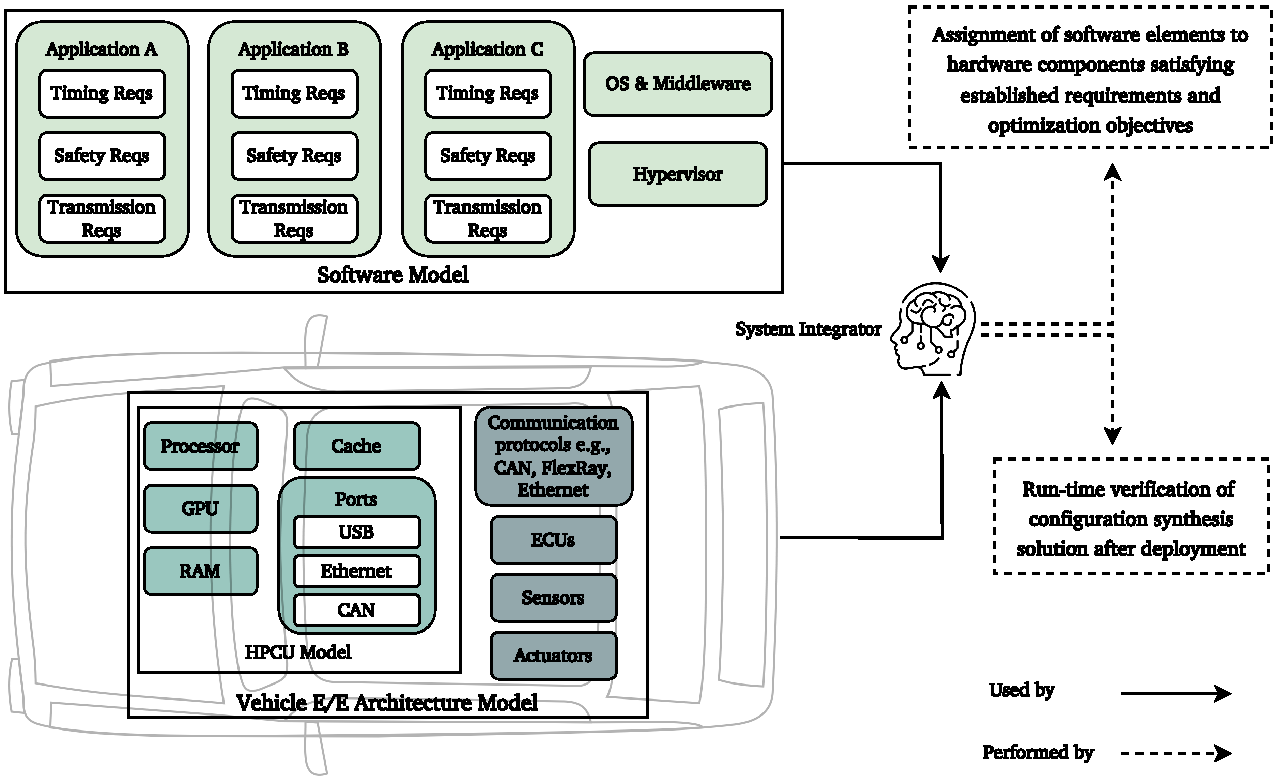
\includegraphics[width=1\columnwidth]{figures/swhw_motiv.pdf}
    \caption{The manual procedures must be executed by a system integrator to create configuration syntheses for automotive software components and the vehicle E/E architecture model.}
    \label{fig0012}
    \end{figure}
    \subsection{Research Questions}
    As explained above, current and future E/E architectures encounter various challenges and bottlenecks, including configuration synthesis for software and hardware of the vehicles, as illustrated in Subsection \ref{motiv}. Making the synthesis of E/E architectures semi-automated or automated facilitates the whole synthesis process and reduces the design process's effort, possible design mistakes, and complexity. Also, it helps to avoid undesired functional safety violations. This can be achieved by using computer-assisted software tools. 
    Following this motivation, it aims to answer two research questions related to the automated configuration synthesis of a car's E/E architecture. 
    
    \begin{itemize}
    
        \item How to facilitate design and synthesis of E/E architectures? 
        
        %As stated in the subsection~\ref{motiv}, the design and configuration synthesis of vehicle E/E systems are complex and time-consuming that demand domain-specific knowledge. Specially when the number of requirements and optimization and boundary objectives increases. The type of synthesis problems such as time-triggered scheduling, message routing, and mapping or resource allocation are also important since, for instance, finding feasible time-triggered schedules is a NP-complete problem. Tool-assisted approaches simplify the design and configuration synthesis of E/E systems. In the current state of the art, there are many commercial/non-commercial tools for modeling and synthesizing of E/E architectures and automotive embedded systems as are described in Chapter~\ref{sota}. Various hardware/software properties, safety/non-safety requirements, synthesis problems, and optimization objectives can be considered to design and synthesize car's E/E architectures. 
        %As mentioned in subsection~\ref{motiv}, the design and configuration synthesis of vehicle E/E systems are complex and time-consuming, demanding domain-specific knowledge, especially when dealing with a growing number of requirements, optimization objectives, and boundary constraints. The specific type of synthesis problems, such as time-triggered scheduling, message routing, and mapping or resource allocation, is also crucial. For instance, finding feasible time-triggered schedules is an NP-complete problem.
        
        
        %To handle these challenges in the design phase, tool-assisted approaches are considered which simplify the design and configuration synthesis of E/E systems. In the current state of the art, there is a plethora of both commercial and non-commercial tools available for modeling and synthesizing E/E architectures and automotive embedded systems, as detailed in Chapter~\ref{sota}. These tools can accommodate various hardware and software properties, safety and non-safety requirements, synthesis problems, and optimization objectives to facilitate the design and synthesis of car E/E architectures.
        
        As mentioned in Subsection~\ref{motiv}, the design and configuration synthesis of vehicle E/E systems are complex and time-consuming, demanding domain-specific knowledge, particularly when faced with increasing requirements, optimization objectives, and boundary constraints. Specific synthesis problems, such as time-triggered scheduling, message routing, and mapping or resource allocation, are also of critical importance. For example, finding feasible time-triggered schedules is an NP-complete problem.


        Tool-assisted approaches can be utilized to address these challenges in the design phase, simplifying the design and configuration synthesis of E/E systems. In the current state of the art, a plethora of commercial and non-commercial tools are available for modeling and synthesizing E/E architectures and automotive embedded systems, as elaborated upon in Chapter~\ref{sota}. These tools can accommodate various hardware and software properties, safety and non-safety requirements, synthesis problems, and optimization objectives, thereby facilitating the design and synthesis of car E/E architectures. However, they have limitations regarding the diversity of synthesis problems, optimization goals, and safety and non-safety requirements.
        
        The process involves gathering relevant information for synthesis problems and selected requirements and objectives, realizing them, transforming them into mathematical constraints, and solving them to find optimized solutions using solvers. 
        
        
        %All necessary steps are required for extracting related information for synthesis problems and selected requirements and objectives by the user, realizing them, transforming them into mathematical constraints, and solving the constraints and finding the optimized solutions by the solvers.
        %In the tools with support of design space exploration, All requirements are automatically transformed into constraints that represent the mathematical formulation of various synthesis problems, requirements, and optimization goals, after collecting and analyzing architectural requirements based on the user design. All these constraints are then solved and optimized by solvers.
         
         
         %the mapping, message routing, safety, and scheduling requirements using integer linear programming (ILP). This transformation is done using the model driven development (MDD) approach~\cite{selic2003pragmatics}. The  set of constraints is then solved in a single step using single-step solving algorithms based on predefined optimization goals.
        
        
        
        \item How to simplify analysis of design errors in E/E architectures?
        
             %Having always feasible solutions for design of E/E systems is not possible. E/E architects can model E/E architectures while selecting various specified requirements and optimization goals. After solving of the designed E/E models, sometimes the solver concludes that there are no feasible solutions. This happens due to the existing conflicts within the constraints system. The origin of the violation must be identified to correct the errors and the make the system model feasible. This action becomes extremely time-consuming and complex when there are a significant number of constraints within the system model. Therefore, an approach is needed to address this issue so that the violated constraints can be recognized faster in order to make the system model satisfiable.
             
            Ensuring that there are always feasible solutions for the design of E/E systems is not guaranteed. E/E architects can model E/E architectures while selecting various specified requirements and optimization goals. However, after solving the designed E/E models, sometimes the solver concludes that no feasible solutions exist. This occurs due to conflicts within the constraints system. Identifying the source of the violation is necessary to correct the errors and make the system model feasible. This process becomes exceedingly time-consuming and complex when there are many constraints within the system model. Thus, an approach is needed to address this issue, enabling the identification of violated constraints more quickly to make the system model satisfiable.     
             
        
        	%To address this challenge, a methodology for identifying violated constraints can assist E/E system architects in identifying the source of conflicts much earlier in the design process, thereby enabling them to navigate towards a feasible solution more efficiently.
        
        %\item
    \end{itemize}
    
    
    
    %\section{Contributions}
    
    
    
    
    
    
    \section{Thesis Contributions}
    
    	%Based on the first research question, automation in simplifying the design and synthesis of car E/E architecture plays a pivotal role. To contribute to this question a model-based software framework is presented. As mentioned, there are many tools for modeling and synthesizing the E/E systems, but they have their own limitations in various aspects such covered synthesis problems, safety requirements, optimization goals, etc. as will be expressed in details in Chapter~\ref{sota}. 
    	Addressing the first research question, automation is pivotal in simplifying the design and synthesis of car E/E architecture. To contribute to this question, we present a model-based software framework. While numerous tools are available for modeling and synthesizing E/E systems, they often come with limitations in areas such as synthesis problems, safety requirements, optimization goals, and more. These limitations are comprehensively analyzed in the literature review in Chapter~\ref{sota}. 
    	
    	
    	
    	
    	Therefore, the introduced modeling tool offers new features including automatic mapping/resource allocation for multi-core computing units and software and hardware components, automatic creation of various types of communication message routings for automotive networks, and the computation of time-triggered schedules for application threads and communication tasks. %All the aforementioned synthesis problems are solved in a single-step in order to reduce the solving time and respect the interrelations between the defined constraints. The framework benefits from the algorithms which makes this goal possible.
    	These synthesis problems are all addressed in a single step to reduce solving time and account for the interrelations between defined constraints. The framework leverages advanced algorithms to achieve this goal.
	    %The presented tool also covers various safety requirements while solving the problems such as FFI, ASIL level, reliability, redundancy, and homogeneous redundancy. Moreover, it supports various optimization goals and boundary conditions comprising end-to-end latency, response time, resource utilization including memory and processor, link occupation rate (LOR), bandwidth usage, and cost of model components. These terms are explained in Chapters~\ref{basicConcepts} and \ref{method}.
	    Furthermore, the presented tool encompasses a wide range of safety requirements, including FFI, ASIL considerations, reliability, redundancy, and homogeneous redundancy. It also caters to various optimization goals and boundary conditions, such as end-to-end latency, response time, resource utilization (including memory and processor), link occupation rate (LOR), bandwidth usage, and E/E components cost. Detailed explanations of these terms can be found in Chapters~\ref{basicConcepts} and \ref{method}.
	    
	    
	
	    %To develop this framework, a model driven development (MDD) approach is used where an object-oriented metamodel is developed which builds the basis of all defined synthesis problems, requirements, optimization objectives, and boundary constraints. To implement the all these features discussed above as form of constraints, the linear programming is utilized. The complexity of linear programming becomes invisible for system integrators or E/E system architects by developing an object-oriented graphical modeling tool as the frontend of the framework. Hence, the E/E architectures consisting of hardware and software components can be modeled. The modeler provides different features for the user such as drag \& drop and automatic creation of hardware/software components functionalities which make the modeling simpler.
	    
	    
        To develop this framework, we employ a model-driven development (MDD) approach, wherein an object-oriented metamodel serves as the foundation for all defined synthesis problems, requirements, optimization objectives, and boundary constraints. Linear programming is utilized to implement all the features discussed above in the form of constraints. The complexity of linear programming is hidden from system integrators and E/E system architects by creating an object-oriented graphical modeling tool as the frontend of the framework. As a result, E/E architectures, comprising hardware and software components, can be easily modeled. The modeler offers various user-friendly features such as drag-and-drop functionality and automatic hardware/software components creation, simplifying the modeling process.
	    
	    
	    
	    
	    
	    %After the modeling step, all logical requirements and properties are collected and they build the E/E system knowledge database. The created database is used for generating the constraints related to the above-mentioned problems and goals. The constraints are solved and optimized by a solver to produce an optimized configuration synthesis for the designed model. All details regarding the methodology and approach of the presented framework are illustrated in Chapter~\ref{method}.
	    Once the modeling step is complete, all logical requirements and properties are collected to build the E/E system knowledge database. This database is then used to generate constraints related to the previously mentioned problems and goals. A solver subsequently solves and optimizes these constraints, resulting in an optimized configuration synthesis for the designed model. The methodology and approach used in the introduced framework are explained in Chapter~\ref{method}.
	    %The solution is fused to the frontend in order to be observable by the user. All frontend details are discussed in Chapter~\ref{frontend}. 
	    The solution is integrated into the frontend to be accessible and observable by the user. The details of the frontend are addressed in Chapter~\ref{frontend}.
	    
	    
	   %To evaluate the developed software tool, various evaluation schemes are employed including the design-time evaluation, which focuses on tool's performance, applicability, and scalability in design phase by using diverse case studies, run-time evaluation, which solutions created by the tool are deployed on a real hardware platform, and qualitative and quantitative evaluation which presents the performance, usability, and practicality of the framework by modeling and synthesizing a series of use cases once manually and once using the introduced tool. The evaluation part is presented in Chapter~\ref{eval}. To discuss the first research question, Chapters \ref{sota}, \ref{method}, \ref{frontend}, and \ref{eval} are expressed. 
	
         Various evaluation schemes are employed to evaluate the developed software tool, as described in Chapter~\ref{eval}. These include:
         
         \begin{itemize}
             \item Design-time evaluation: This assessment focuses on the tool's performance, applicability, and scalability during the design phase. It involves using diverse case studies to test the tool's capabilities.
             
             \item Run-time evaluation: In this phase, solutions created by the tool are deployed on a real hardware platform to assess their practical performance.
             
             \item Qualitative and quantitative evaluation: This approach examines the tool's performance, usability, and practicality. It involves modeling and synthesizing a series of use cases performed by multiple users, both manually and using the introduced tool.
         
         \end{itemize}
         To address the first research question, Chapters \ref{method}, \ref{frontend}, and \ref{eval} are introduced.	    
	
	
	
	%Following the second research question, when feasible solutions cannot be navigated by the solver, the solutions become unsatisfiable or infeasible which are common while solving a constraint system.This occurs due to the conflicts between constraints in the system model.
	%Navigating the source of violation can be time-consuming and complex, and it gets much worse when a huge number of constraints exists in the system model. As a result, an approach is presented in Chapter~\ref{designerror} to identify design errors or source conflict between constraints after the solving process. In this approach, two different methods are utilized to produce minimal set of unsatifiable constraints and cores. The proposed approach uses these methods to identify the most critical constraints which cause the model infeasibility. Based on the introduce approach, a list of constraints is created, each of these constraints includes an assigned weight. The assigned weight is proportional to the number of times it has been identified as a cause of model unsatisfiability. Therefore, the system integrator is able to find the origin of conflicts between constraints using the weighted constraints. In addition, the model can become satisfiable after correcting the source of violation. 
	
	
		%In response to the second research question, when feasible solutions cannot be navigated by the solver, the solutions become unsatisfiable or infeasible which are common while solving a constraint system.
	In response to the second research question, when a solver cannot find feasible solutions, these solutions become unsatisfiable or infeasible, which is common when solving a constraint system.
	This arises from the conflicts between constraints within the system model.
	Identifying the source of violation can be time-consuming and complex, especially when dealing with many constraints within the system model. To address this challenge, an approach is presented in Chapter~\ref{designerror} for identifying design errors or pinpointing conflicts between constraints after the solving process. This approach uses two distinct methods to generate a minimal set of unsatisfiable constraints and cores. 
	The proposed approach then utilizes these methods to identify the most critical constraints responsible for model infeasibility.  As part of this approach, a list of constraints is created, with each constraint assigned a weight proportional to the number of times it has been identified as the cause of model unsatisfiability.
	Consequently, using these weighted constraints, the system integrator can pinpoint the origins of conflicts between constraints. Furthermore, it is possible to make the model satisfiable again by addressing and correcting the source of the violation.
	%The proposed approach uses these methods to identify the most critical constraints which cause the model infeasibility.
	%Based on the introduced approach, a list of constraints is created, each of these constraints includes an assigned weight. The assigned weight is proportional to the number of times it has been identified as a cause of model unsatisfiability.
	%Therefore, the system integrator is able to find the origin of conflicts between constraints using the weighted constraints. In addition, the model can become satisfiable after correcting the source of violation. 
	%In Chapter~\ref{designerror}, evaluations of different scenarios for the introduced approach are discussed. Each stated method is assessed separately; however, one method is considered as the main one in the presented approach as it is compatible with the solver utilized in the tool.  
	In addition, in Chapter~\ref{designerror}, evaluations of various scenarios for the design error analysis approach are discussed. Each method is assessed individually. However, one particular method is considered the primary approach in this presentation, primarily due to its compatibility with the solver used in the tool. 
	
	Most of this thesis's content has been published in various international journals and conferences. In addition, the proposed software framework has become open-source and accessible on GitHub~\cite{askaripoor2023designer}, offering the research community an opportunity to explore, utilize, and contribute to its development. It is believed that open sourcing the introduced tool is essential for fostering collaboration, reproducibility, and transparency in research.
    The most relevant publications are as follows.
    
    
    \begin{itemize}
    
        \item H. Askaripoor, T. Mueller and A. Knoll, "E/E Designer: a Framework to Design and Synthesize Vehicle E/E Architecture," in IEEE Transactions on Intelligent Vehicles, doi: 10.1109/TIV.2023.3324617.
        
        \item Askaripoor, H., Hashemi Farzaneh, M. and Knoll, A., 2022. E/e architecture synthesis: Challenges and technologies. Electronics, 11(4), p.518.
        
         \item Askaripoor, H., Farzaneh, M.H. and Knoll, A., 2021, September. A model-based approach to facilitate design of homogeneous redundant e/e architectures. In 2021 IEEE International Intelligent Transportation Systems Conference (ITSC) (pp. 3426-3431). IEEE.
        
         \item Askaripoor, H., Farzaneh, M.H. and Knoll, A., 2021, September. A platform to configure and monitor safety-critical applications for automotive central computers. In 2021 26th IEEE International Conference on Emerging Technologies and Factory Automation (ETFA) (pp. 1-4). IEEE.
        
        \item Askaripoor, H., Farzaneh, M.H. and Knoll, A., 2020, September. Considering safety requirements in design phase of future e/e architectures. In 2020 25th IEEE International Conference on Emerging Technologies and Factory Automation (ETFA) (Vol. 1, pp. 1165-1168). IEEE.
        
        \item Askaripoor, H., Shafaei, S. and Knoll, A., 2021. A flexible scheduling architecture of resource distribution proposal for autonomous driving platforms. In Proceedings of the 7th International Conference on Vehicle Technology and Intelligent Transport Systems.
        
        \item T. Müller, H. Askaripoor and A. Knoll, "Advancing E/E Architecture Synthesis: A Perspective on Reliability Optimization and Hypervisor Integration," 2024 IEEE Intelligent Vehicles Symposium (IV), Jeju Island, Korea, Republic of, 2024, pp. 1996-2003, doi: 10.1109/IV55156.2024.10588416. 
        
        \item Müller, T., Askaripoor, H. and Knoll, A., 2022, October. Performance analysis of KVM hypervisor using a self-driving developer kit. In IECON 2022–48th Annual Conference of the IEEE Industrial Electronics Society (pp. 1-7). IEEE.
        
    \end{itemize}
    
    
    
    %Our study presents a model-based framework that simplifies the synthesis of vehicle E/E architectures and reduces the effort and complexity of the design process for multi-core embedded systems and communication networks used in the vehicle's E/E architecture. It supports the automated mapping of software components such as applications, processes, and threads to hardware components e.g., processors, cores, ECUs, etc. for multi/many-core embedded systems. It also calculates time-triggered schedules for the processes and threads assigned to a specific core/processor for real-time applications. In addition, \textit{E/E Designer} automatically generates network message routings for the vehicle communication network and computes time-triggered schedules for each predefined communication task routed over a network link. Furthermore, various safety requirements and optimization objectives are covered by \textit{E/E Designer}. 
    
    
    %This framework consists of a back end and a front end. In the framework's back-end, after collecting and analyzing architectural requirements based on the user design in the front-end, all requirements are automatically transformed into constraints that represent the mathematical formulation of the mapping, message routing, safety, and scheduling requirements using integer linear programming (ILP). This transformation is done using the model driven development (MDD) approach~\cite{selic2003pragmatics}. The  set of constraints is then solved in a single step using single-step solving algorithms based on predefined optimization goals. The result includes optimized mapping, message routing, and time-triggered schedules for the designed E/E architecture. Moreover,to evaluate the performance of this framework, two types of experiments are proposed. First, design-time evaluation which the synthesis time of \textit{E/E Designer} is measured for different use cases. Second, run-time evaluation as presented in our work-in-progress paper~\cite{9613692}, where the design-time solutions comprising mapping, scheduling, and message routing made by \textit{E/E Designer} are deployed on an experimental setup including three different hardware performing various evaluation metrics such as jitter, response time, end-to-end latency, temperature, central processing unit (CPU), and random access memory (RAM) measurements. 
    
    
    %Overall, the goal of this work is to create more efficient and reliable message routing for automotive networks, which are becoming increasingly complex as more features and sensors are added to modern vehicles. The proposed approach aims to simplify the process of creating routing configurations, while also improving the redundancy and fault tolerance of the system.
    

    
    \section{Thesis Structure}
    
    The thesis is structured as follows. 
    
    \begin{itemize}
        \item  %The basic concepts and terms are discussed in Chapter~\ref{basicConcepts} where various concepts and terminologies regrading resource allocation, time-triggered scheduling, message routing in automotive networks, vehicle communication protocols, automotive safety standards, safety requirements relevant to this thesis, and virtualization technologies, are presented. 
        The fundamental concepts and terms are elaborated upon in Chapter~\ref{basicConcepts}, where a range of topics, including resource allocation, time-triggered scheduling, message routing in automotive networks, vehicle communication protocols, automotive safety standards, safety requirements relevant to this thesis, and virtualization technologies, are discussed.
        
        
        \item  %In Chapter \ref{sota}, a comprehensive analysis of state of the art is illustrated. The analysis focuses mostly on automotive software architecture synthesis-related studies, technologies and frameworks/tools for modeling and synthesizing E/E systems and software integration and configuration in design process. It also covers studies regarding mapping problem, communication message routing, and time-triggered scheduling. In the final section of this chapter, a discussion and summary are presented.  
       In Chapter \ref{sota}, a comprehensive analysis of the state of the art is presented. This analysis primarily focuses on studies related to automotive software architecture synthesis, technologies, and frameworks/tools for modeling and synthesizing E/E systems, as well as software integration and configuration in the design process. Additionally, it encompasses research on mapping problem, communication message routing, and time-triggered scheduling. The final section of this chapter includes a discussion and summary.
        
        \item  %The approach of proposed framework is explained in Chapter~\ref{method}. This chapter includes various sections such as framework architecture, framework system model, and constraints MIP formulation. Moreover, it discusses boundary constraints and optimization objectives, multi-objective optimization, single-step solving algorithms, constraint formulation as mixed integer programming for Gurobi optimization solver, and discussion sections. 
       The approach of the proposed framework is explained in Chapter~\ref{method}. This chapter includes various sections, such as framework architecture, framework system model, and mixed-integer programming (MIP) formulation of constraints. Moreover, it discusses boundary constraints, optimization objectives, multi-objective optimization, single-step solving algorithms, and constraint formulation for the Gurobi optimization solver and provides a discussion section \cite{gurobi}.
        
        \item %The frontend of the proposed software tool is explained in Chapter~\ref{frontend}. This chapter consists of modeling, requirements and properties, solving and solutions, model validation, and implementation sections.
        The frontend of the proposed software tool is detailed in Chapter~\ref{frontend}, which comprises sections on modeling, requirements and properties, solving and solutions, model validation, and implementation.
        
        \item %Chapter~\ref{designerror} explains the approach for identifying design errors when violations happen in the constraint set after its solving.  It comprises background, approach, and evaluation sections.
        In Chapter~\ref{designerror}, the approach for identifying design errors when violations occur in the constraint set after it has been solved is explained. This chapter involves background, approach, and evaluation sections.
        
        \item %The performance of the introduced software framework is evaluated in Chapter~\ref{eval}. This chapter discusses design-time, run-time, and quantitative and qualitative evaluations. 
        The performance of the introduced software framework is assessed in Chapter~\ref{eval}, covering design-time, run-time, and both quantitative and qualitative evaluations.
        
        \item  %Finally, in Chapter~\ref{conclusion}, the conclusion and possible future works of this thesis are expressed.
        %In Chapter~\ref{conclusion}, the thesis concludes and explores possible future work.
        In Chapter~\ref{conclusion}, the thesis conclusion, its limitations, and potential avenues for future research are discussed.
        
    \end{itemize}
    
    %\null
    %\addtocounter{page}{-1}
    %\newpage
    %\thispagestyle{empty}
    
    


    
    
    
  
    
    
    
    %Furthermore, the design of automotive E/E architecture using ADAS functionalities and algorithms, comprising all their safety and non-safety-critical requirements, is an elaborate and time-consuming task that requires domain-specific knowledge~\cite{9565115}. Moreover, manual integration and configuration of the software architecture for an automotive central high-performance computer, while satisfying all safety essentials, is a challenging and error-prone task because of the high number of requirements and properties related to hardware, the applications, operating system (OS), middleware, hypervisor, etc. Such configurations can be optimized as well by determining various optimization goals such as power consumption, resource utilization, reliability, temperature, and others. Therefore, approaches/tools, in order to automate the software configuration process during the design-time while taking all requirements and properties into account, can cope with growing complexity, and facilitate and improve the design process focused on modeling and mapping of software components on the automotive high-performance computing unit (HPCU).
    
    %In recent years, as the level of vehicle automation (such as ADAS) has increased, the demand for computational power in vehicle ECUs has grown dramatically. Currently, cars are equipped with anywhere from 70 to 100 ECUs to manage their software systems \cite{pelliccione2017automotive}.
    
    %However, this number of ECUs could be significantly reduced by merging multiple mixed-critical applications into a single multi-core ECU. Figure.\ref{fig3} depicts the configuration processes that must be carried out by a system architect during both design and run-time in order to find a mapping solution that deploys mixed-critical software components to the HPCU while taking into consideration their properties and configuration parameters, the safety-critical/non-critical requirements of the applications, and optimization objectives. Furthermore, the system architect must also verify that the requirements have been met in run-time due to the unpredictable behavior of the operating system, middleware, and applications (as shown in Fig.\ref{fig3})~\cite{askaripoor2021flexible}.
    
    %However, the process of designing these configurations and mappings is extremely complex and challenging~\cite{9212001},\cite{zheng2016next}. Furthermore, the problem of finding the configuration can become a non-deterministic polynomial-time (NP)-hard problem, depending on the mapping problem(\cite{singh2016resource,sahu2013survey,mehrara2009multicore}), due to the vast number of safety-critical/non-critical application and user requirements, e.g., reliability~\cite{xie2017fast}, timing, latency, worst-case execution time, central processing unit (CPU) utilization, bandwidth, memory usage, power consumption, FFI, automotive safety integrity (ASIL) level~\cite{xie2020recent}, redundancy, etc., the expansive design space of possible task mappings, and the non-deterministic/dynamic workload.
    %Furthermore, with the increase in number of applications and components including their requirements and properties, discovering the configuration and mapping solution becomes more and more complex for the system architect, and the need to have a new update in the configuration might lead to unknown risks and become costly (See Fig.~\ref{fig3})~\cite{9613692}. 
    %Additionally, as the number of applications and components continues to grow, along with their corresponding requirements and properties, the task of finding the ideal configuration and mapping solution becomes increasingly complex for system architects. The need to update the configuration can also introduce unknown risks and result in high costs, as illustrated in Fig.\ref{fig3}\cite{9613692}.
    
    
    %However, developing an automotive E/E architecture with ADAS functionalities and algorithms, considering all safety-related (e.g., timing, freedom from interference (FFI), and redundancy) and non-safety-related requirements, is a laborious and time-consuming task that requires domain-specific knowledge~\cite{9565115,9212001}. Moreover, manual integration and configuration of the software architecture for an automotive high-performance computing unit (HPCU) is a challenging and error-prone task, as a variety of requirements and properties related to hardware, applications, operating system (OS), middleware, hypervisor, etc. must be met. This also applies to the configuration of an automotive communication network, where a reliable data transmission of safety-critical ADAS applications over the network must be enabled. Such configurations can also be optimized by setting various optimization goals such as power consumption, resource utilization, reliability, temperature, cost, response time, end-to-end latency, and others\cite{askaripoor2022architecture}. 
    
    
    
    
    
    
    
    
    %However, being an autonomous vehicle opens a significant number of challenges corresponding to vehicle safety at run-time and design-time. The topology of the architecture has significant impact on various aspects of the car including safety (e.g. redundancy for fail-operational) and cost. Moreover, the design of the vehicle E/E architecture in compliance with functional safety standards is an elaborate task for automotive designers. For example, finding of adequate routes and traffic schedules in architectures with fixed topology are well-known intractable NP-problems~\cite{b36} with an exponential or even over-exponential computations times. It is obvious that the creation of a safe topology increases the complexity of the problem.Our work in progress paper presents a framework under development to generate the architecture topology based on predefined constraints including e.g. route redundancy to facilitate the architecture design procedures of self-driving vehicles.

%Hence, in this paper, we present a work in progress which focus on model based development for creating automotive architecture based on pre-defined rules.   

%\todo  
 %Considering the topology generation is an elaborate issue from mathematical side. So that the number of possible connection that ($n$) nodes can have in a full mesh topology is $O(n!)$  which is a NP problem (non-deterministic polynomial time).


%Recently, zonal Electrical/Electronic architecture is mentioned  as the state of the art vehicle architecture and it could provide several advantages for whole the car hardware and software structure. In this paper, we focus on the safety aspects and characteristics of the zonal E/E architecture in automotive domain.



%\section{Background}



%This paper explains a summary of the evolution of the car E/E architectures describing the main three E/E architecture's types, the current main issues, and the key technologies for the future; in addition, the high-level software architecture of the automotive HPCU is illustrated. Also, it goes through the current challenges for E/E architecture concentrated on software integration and configuration, and the multi-core ECUs. Moreover, it provides an overview regarding task mapping approaches for multi-core computing units. In this study, furthermore, the available approaches and tools for automotive software integration and configuration, and E/E architecture synthesis, focused on mapping problems and modeling of the software components comprising design space exploration(DSE) approaches and optimization goals, are presented. As a result of this technologies analysis, four research questions are depicted as future works in this research area. The analysis result can be useful for other researchers and E/E system architects in the industry in order to assist to automate and facilitate the configuration process of the software components particularly applications for the automotive HPCUs.




%complexity and types of applications required in today's vehicles have increased significantly, particularly with advanced driver assistance systems (ADAS) and self-driving capabilities. In addition, meeting all non-safety and safety-related requirements following automotive standards (i.e., ISO 26262 and safety of intended functionality (SOTIF)) during the early design phase and configuration of automotive software architecture increases the complexity~\cite{sotif},~\cite{iso26262}. Automotive electrical and/or electronic (E/E) architecture has recently evolved to accommodate the aforementioned complexity resulting from the new applications and functionalities that need to be integrated into the vehicle and the limitations of traditional E/E architectures. The Vehicle E/E architecture started with distributed/decentralized architectures, where a significant number of electronic control units (ECUs) are interconnected, each having a specific vehicle functionality. Then it progressed to domain-centralized, where centralized domain ECUs are used, and to centralized/zonal architectures, where the vehicle architecture relies on zonal controllers~\cite{askaripoor2022architecture}. Concerning ADAS and automated driving, using multi-core computing units is a solution to achieve adequate performance for artificial intelligence (AI)-based applications and reduce complications related to hardware (e.g., wiring harness, and number of ECUs) and software variations. 

%Furthermore, a significant amount of data needs to be transmitted over the in-vehicle communication network due to the new infotainment and driver assistance features. However, high transmission reliability of the networks must be ensured when the vehicle makes safety-critical decisions based on messages over its communication network. In addition, low latency or even deterministic message transmission and correct schedules for each communication frame are required to meet the demands of real-time applications.





%Moreover, we introduce an approach under development to analyze design errors in case of facing infeasible solutions during using \textit{E/E Designer}.


   

%This study is outlined as follows: Section II discusses related work.
%Section III states the background of mapping in multi-core embedded systems, time-triggered scheduling, communication message routing, path dependency in vehicle's network, and safety-related requirements covered by \textit{E/E Designer}. Section IV describes our methodology which consists of the back end (including \textit{E/E Designer} system architecture, system model, constraints formulation, optimization objectives, multi-objective optimization, constraint formulation for Gurobi solver, and constraints solving) and front end (comprising modeling, requirements and properties, solving and solutions, and model validation). Section V, presents the evaluation of \textit{E/E Designer} including design-time and run-time evaluations. Finally, the conclusion and future steps are presented in section VI.












%While the zonal ECU provides and distributes data and power; moreover, it supports any feature available in each specific vehicle zone. It can support any kind of interface for sensors, actuators, and displays. In addition, the zonal ECU behaves as a gateway, switch, and as a smart junction box which is scalable










%\section{Technologies and Challenges}\label{challenge}
%In the last years, with increasing the level of the vehicle automation (e.g., ADAS) the need for computational power in vehicle ECUs has grown significantly. Current cars are equipped with 70 to 100 ECUs to manage the software system \cite{pelliccione2017automotive}. The number of ECUs could be reduced considerably by merging various mixed-critical applications into one multi-core ECU. Figure.~\ref{fig3} depicts the configuration procedures in design and run-time which are required to be performed by a system architect to find a mapping solution for deploying mixed-critical software components to the HPCU considering their properties and configuration parameters, safety-critical/non-critical requirements of the applications, and optimization objectives. In addition, the system architect must verify the fulfillment of the requirements after solution deployment in run-time because of the unpredictable behavior of OS, middleware, and applications (See Fig.~\ref{fig3})~\cite{askaripoor2021flexible}.

%In recent years, as the level of vehicle automation (such as ADAS) has increased, the demand for computational power in vehicle ECUs has grown dramatically. Currently, cars are equipped with anywhere from 70 to 100 ECUs to manage their software systems \cite{pelliccione2017automotive}. However, this number of ECUs could be significantly reduced by merging multiple mixed-critical applications into a single multi-core ECU. Figure.\ref{fig3} depicts the configuration processes that must be carried out by a system architect during both design and run-time in order to find a mapping solution that deploys mixed-critical software components to the HPCU while taking into consideration their properties and configuration parameters, the safety-critical/non-critical requirements of the applications, and optimization objectives. Furthermore, the system architect must also verify that the requirements have been met in run-time due to the unpredictable behavior of the operating system, middleware, and applications (as shown in Fig.\ref{fig3})~\cite{askaripoor2021flexible}.






%However, designing such configurations and mappings turns out extremely complicated and challenging~\cite{9212001},~\cite{zheng2016next}. Moreover, depending on the mapping problem, finding the configuration may become a non-deterministic polynomial-time (NP)-hard problem~(\cite{singh2016resource,sahu2013survey,mehrara2009multicore}) because of the huge number of safety-critical/non-critical application and user requirements (e.g., reliability~\cite{xie2017fast}, timing, latency, worst-case execution time, central processing unit (CPU) utilization, bandwidth, memory usage, power consumption, FFI, automotive safety integrity (ASIL) level~\cite{xie2020recent}, redundancy, etc.), the extensive design space of possible task mappings, and non-deterministic/dynamic workload. 
%However, the process of designing these configurations and mappings is extremely complex and challenging~\cite{9212001},\cite{zheng2016next}. Furthermore, the problem of finding the configuration can become a non-deterministic polynomial-time (NP)-hard problem, depending on the mapping problem(\cite{singh2016resource,sahu2013survey,mehrara2009multicore}), due to the vast number of safety-critical/non-critical application and user requirements, e.g., reliability~\cite{xie2017fast}, timing, latency, worst-case execution time, central processing unit (CPU) utilization, bandwidth, memory usage, power consumption, FFI, automotive safety integrity (ASIL) level~\cite{xie2020recent}, redundancy, etc., the expansive design space of possible task mappings, and the non-deterministic/dynamic workload.
%Furthermore, with the increase in number of applications and components including their requirements and properties, discovering the configuration and mapping solution becomes more and more complex for the system architect, and the need to have a new update in the configuration might lead to unknown risks and become costly (See Fig.~\ref{fig3})~\cite{9613692}. Additionally, as the number of applications and components continues to grow, along with their corresponding requirements and properties, the task of finding the ideal configuration and mapping solution becomes increasingly complex for system architects. The need to update the configuration can also introduce unknown risks and result in high costs, as illustrated in Fig.\ref{fig3}\cite{9613692}.

%As explained in sections~\ref{current} and~\ref{future}, current and future E/E architectures encounter various challenges and bottlenecks including software integration and configuration for the HPCU. Hence, this paper focuses mainly on software integration and configuration for automotive embedded systems. It firstly expresses the existing approaches and methods for dynamic and static task mappings in multi-core processors considering various optimization goals. Secondly, it discusses the current design-time technologies and approaches for software integration, including model analysis, E/E architecture synthesis, configuration, model checking, and mappingThe current and future E/E architectures as discussed in \textcolor{red}{sections~\ref{current} and~\ref{future}} face numerous challenges and bottlenecks, particularly in the area of software integration and configuration for the HPCU. In light of these challenges, this paper places a strong emphasis on the topic of software integration and configuration for automotive embedded systems. To achieve this goal, the paper firstly examines existing approaches and methods for dynamic and static task mapping in multi-core processors, considering various optimization objectives. Secondly, the paper delves into the current design-time technologies and approaches for software integration, including model analysis, synthesis of E/E architecture, configuration, model checking, and mapping.



 
%In this section, the all existed technologies as well as the challenges regarding the the following sub sections will be expressed.










\begin{comment}


\subsection{The main bottleneckes of E/E Architecture}
There are several bottlenecks that can affect the performance of an electronic/electrical (E/E) architecture in a vehicle. Some of the main bottlenecks include:
Data transfer speed: The speed at which data can be transferred between components within the E/E architecture can be a bottleneck, particularly if the architecture relies on a central network to connect all components. This can be mitigated by using high-speed communication protocols such as Ethernet or by implementing distributed architecture designs that reduce the need for data to be transferred between components.
Processor speed and memory: The speed of processors and the amount of memory available can also be bottlenecks if the system is required to perform complex tasks or handle large amounts of data. Upgrading to faster processors or increasing the amount of memory can help to mitigate these bottlenecks.
Power management: Ensuring that the E/E architecture has sufficient power to meet the demands of the various components can be a challenge, particularly in systems that require high levels of power. Implementing effective power management strategies, such as power-saving modes or intelligent power distribution, can help to mitigate these bottlenecks.
System integration: Integrating different components and systems within the E/E architecture can be a bottleneck if there are compatibility issues or if the integration process is not well-managed. Using standardized communication protocols and following best practices for system integration can help to mitigate these bottlenecks.


\section{Future Research Areas}\label{future}

There is a demand to simplify the integration process for automotive OEMs and third-party developers. In other words, simplifying the offline software integration process by semi-automating and automating the integration of the safety-critical applications in next-generation automotive central compute platforms. As illustrated in section \ref{challenge}, designing the configurations and mappings for the HPCUs, while fulfilling all safety requirements and considering optimization goals, is a challenging and time-consuming task. Furthermore, as the number of applications and their requirements increase exploring a mapping solution becomes NP. 

Current manual and offline integration processes are not ready for the needs of next-generation automotive HPCUs. As studied in this paper, there are various frameworks and approaches which contribute to semi-automate the integration and mapping process for embedded systems and HPCUs. However, none of these studies or platforms fully automate the integration and mapping process for multi-core computing units. In addition, there are a significant number of safety requirements based on automotive safety standards which have not been discussed in the previously mentioned studies.  
Moreover, as illustrated in Figure~\ref{fig3}, deploying the mapping solution on an HPCU plays a critical role in evaluating the performance of the solution in run-time in terms of predefined optimization objectives in design-time and study the run-time behavior of the OS and applications to improve the mapping outcome created by the design-time framework. More importantly, verifying all constraints and requirements, which are defined in the design-time approach, after solution deployment on the HW in the run-time is another major criterion to ensure the functionality of the created configuration solution in the running phase.  

After the DSE method is utilized to find the optimal mapping solution, there is a probability that the user receives an infeasible solution as the output of the solver because of conflicts in the constraints system. Therefore, proposing an approach to provide a capability to identify the source of the violation in the constraints system of the whole system model is extremely important for determining the feasibility of the solution. Otherwise, when the number of constraints increases, finding the violated constraints will be extremely challenging and time-consuming without any clues from which constraint equation they stem. None of the above-discussed frameworks or studies support this capability. Thus, we state the following research questions for the automotive software integration for HPCUs focused on the mapping based on the above-noted explanation. 

\begin{itemize}
    \item How to facilitate and automate the assignment of HPCU resources to safety-critical applications while verifying the satisfaction of the specified safety requirements in the design phase to compute a verified and optimized mapping configuration considering the predetermined optimization objectives?
    \item How to verify the fulfillment of the specified requirements (particularly safety-critical ones) after deployment of the derived configuration to the HPCU at run-time?
    \item How to evaluate the performance of the calculated mapping configuration at run-time focused on the specified optimization goals in design-time?
    \item How to discover the source of the conflict among defined constraints in our system while using the DSE approach to find the optimal solution in case of an infeasible solution? 
\end{itemize}

\end{comment}










